\chapter{Basis and modelling}
\section{UAV model}
A \gls{uav} model is presented in \citep{beard2012small}, which present the kinetic equations of a general MAV in the. The kinetic equations is given in the body frame, which is fixed to the frame of the \gls{uav}. The kinematics equations is given as:
\begin{subequations}
\label{eq:kinematics}
\begin{align}\label{eq:kinematicsPosition}
& \begin{bmatrix}
\dot{x} \\
\dot{y} \\
\dot{z}
\end{bmatrix}
=
 \mathbf{R}(\mathbf{\Theta})_{Body}^{NED}\begin{bmatrix}
 u \\
 v \\
 w
 \end{bmatrix} \\
& \begin{bmatrix}
\dot{\phi} \\
\dot{\theta} \\
\dot{\psi}
\end{bmatrix}
= 
\mathbf{T}(\mathbf{\Theta}_{nb})\begin{bmatrix}
p \\
q \\
r
\end{bmatrix}\label{eq:kinematicsAttitude}
\end{align}
\end{subequations}
where $\mathbf{R}(\mathbf{\Theta})_{Body}^{NED}$ is the rotation matrix from the body frame to the NED frame, with $\mathbf{\Theta} = \begin{bmatrix}
\phi & \theta & \psi
\end{bmatrix}^T.$ The transformation matrix $\mathbf{T}(\mathbf{\Theta}_{nb})$ is given in \citep{fossen2011handbook} as:
\begin{equation}
\mathbf{T}(\mathbf{\Theta}_{nb}) = \begin{bmatrix}
1 & \sin(\phi)\tan(\theta) & \cos(\phi)\tan(\theta) \\
0 & \cos(\phi) & -\sin(\phi) \\
0 & \frac{\sin(\phi)}{\cos(\theta)} & \frac{\cos(\phi)}{\cos(\theta)}
\end{bmatrix}
\end{equation}
The kinetic equations is given as:
\begin{subequations}
\label{eq:kinetics}
\begin{align}
\begin{bmatrix}
F_x \\
F_y \\
F_z
\end{bmatrix}
&= \mathbf{R}(\mathbf{\Theta})^{Body}_{NED}\begin{bmatrix}
0 \\
0 \\
mg
\end{bmatrix} - \frac{1}{2} \rho V_a^2 S \mathbf{R}(\alpha)_{Stability}^{Body}\begin{bmatrix}
F_{Drag} \\
0 \\
F_{Lift}
\end{bmatrix}\\ &+ \frac{1}{2} \rho V_a^2 S \begin{bmatrix}
0 \\
C_y(\beta,p,r,\delta_a,\delta_r) \notag\\
0
\end{bmatrix} + \frac{1}{2} \rho S_{Prop} C_{Prop} \begin{bmatrix}
(K_{Motor}\delta_t)^2-V_a^2 \\
0 \\
0
\end{bmatrix}\\
\begin{bmatrix}
 L \\
 M \\
 N 
 \end{bmatrix} &= \frac{1}{2} \rho V_a^2S\begin{bmatrix}
 C_L(\beta,p,r,\delta_a,\delta_r) \\
 C_M(\alpha,q,\delta_e) \\
 C_N(\beta,p,r,\delta_a,\delta_r)
 \end{bmatrix} + \begin{bmatrix}
 -k_{T_p}(K_\Omega\delta_t)^2 \\
 0 \\
 0
 \end{bmatrix}
\end{align}
\end{subequations}
where $\rho$ is the air density in $kg/m^3$,$mg$ is the weight of the \gls{uav}, $S$ is the platform area of the MAV wing, $C_i$ is nondimensional aerodynamic coefficients and $V_a$ is the speed of the MAV through the surrounding air. $\alpha$ and $\beta$ is the attack and side slip angle respectfully. $F_{Drag}$ is the drag force acting on the fuselage, and $F_{Lift}$ is the lift force. $\mathbf{R}(\alpha)_{Stability}^{Body}$ is the rotation matrix from the stability frame to the body frame. The stability frame is orientated with respect to the MAV movement through the surrounding air, which is defined as a standard rotation around the y-axis of the body frame. $S_{Prop}$ is the area swept out by the propeller, and $K_{Motor}$,$K_{T_p}$ and $K_\Omega$ is propeller specific constants. The control surface on the MAV is defined into two groups; the wings and the rudder. On the rudder $\delta_e$ controls the elevator deflection and $\delta_r$ the rudder deflection. For the wings $\delta_a$ is the control input from the aileron deflection. The control input for the control input is $\delta_t$.
\section{Landing path modelling}
A landing path is a path following problem where the minimum requirement is that the path is connected, and is flyable. The connection level can be described by the paths smoothness. Smoothness can be described with parametric continuity, which is denoted $C^n$ were n is the degree of smoothness. The order of n implies that the n first parametric derivatives match at a common point for two subsequent paths \citep{barsky1989geometric}. Geometric continuity is a relaxed from of parametric continuity in which discontinuousness in speed is allowed. A table \ref{TB:SmoothnessDescriptions} of geometric and parametric continuity lists the requirement for each smoothness level, which is based definitions presented in \citep{barsky1989geometric}.
Geometric continuity is sufficient for a path following system, which is the main focus of this thesis. Geometric continuity is denoted as $G^n$ were n is the order of continuity.

\begin{table}[H]
\begin{center}
\begin{tabular}{| l | l |}
\hline
\textbf{Geometrical smoothness level} & \textbf{Description} \\ \hline
$G^0$ & All subpaths are connected \\ \hline
$G^1$ & The path-tangential angle is continuous \\ \hline
$G^2$ & The center of curvature is continuous \\ \hline
\textbf{Parametric smoothness level} & \textbf{Description} \\ \hline
$C^0$ & All subpaths are connected \\ \hline
$C^1$ & The velocity is continuous \\ \hline
$C^2$ & The acceleration is continuous \\ \hline
\end{tabular}
\end{center}
\caption{Smoothness definitions}
\label{TB:SmoothnessDescriptions}
\end{table} 

The definition used for path in this thesis is equation 1.2 in \citep{tsourdos2010cooperative} which state:
\begin{equation}
P_s(x_s,y_s,z_s,\theta_s,\psi_s) \xrightarrow{r(\varpi)} P_f(x_f,y_f,z_f,\theta_f,\psi_f)
\end{equation}
where the subscripts $s$ and $f$ denotes the start pose and finish pose respectfully with $r(\varpi)$ as the path and $\varpi$ the path variable.

\subsection{Straight lines}
The simplest form on path is a straight line between $P_s$ and $P_f$. For simplicity the path is reduced to a 2 dimensional case, where the straight line is given as 
\begin{subequations}
\begin{align}
& x(\varpi) = a_x\varpi + b_x \\
& y(\varpi) = a_y\varpi + b_y 
\end{align}
\end{subequations}
with $ \varpi \in [0,1] $, where $\varpi$ has not necessary a physical meaning. Then the parametrisation of the straight line is:
\begin{subequations}
\begin{align}
P(0) &= \begin{bmatrix}
x(0) \\
y(0)
\end{bmatrix} = \begin{bmatrix}
b_x \\
b_y
\end{bmatrix} = \begin{bmatrix}
x_s \\
y_s
\end{bmatrix} \\
P(1) &= \begin{bmatrix}
x(1) \\
y(1)
\end{bmatrix} = \begin{bmatrix}
a_x + b_x \\
a_y + b_y
\end{bmatrix} = \begin{bmatrix}
x_f \\
y_f
\end{bmatrix} \rightarrow \begin{bmatrix}
a_x \\
a_y
\end{bmatrix} = \begin{bmatrix}
x_f - b_x \\
y_f - b_y
\end{bmatrix}
\end{align}
\end{subequations}
The tangential vector for a straight line is given as:
\begin{equation}
\psi(\varpi) = \atan2(a_y,a_x)
\end{equation}
with it's derivative:
\begin{equation}
\dot{\psi}(\varpi) = 0
\end{equation}
A path constructed by straight lines is $G^0$, however since the tangential vectors derivative is zeros, it is discontinuous between two line segments with different heading and therefore not $G^1$[TODO: LEGG INN FIGUR SOM VISER DISKONINUITETEN]. The disadvantage with a path which is $G^0$ is that large discontinuity between two tangential vectors will cause problem for a control system. 
\begin{figure}[H]
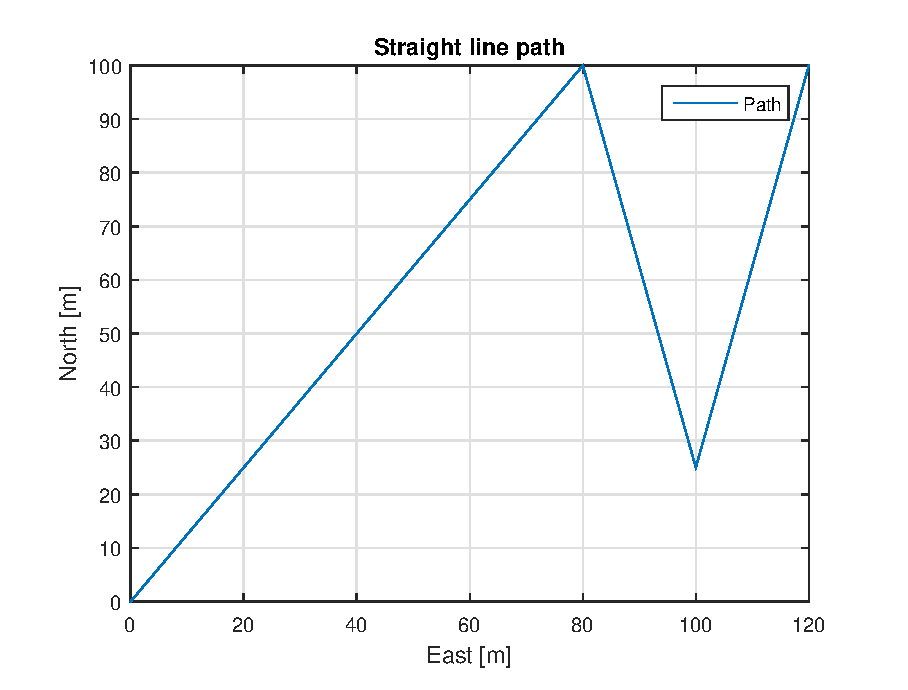
\includegraphics[width=0.7\textwidth]{figs/TheoryPlot/StraightLine.eps}
\caption{Straight line path}
\end{figure}
\subsection{Dubins path}\label{S:DubinsPath}
An alternative to a straight line path is a path constructed by straight lines and circle. Such a path is Dubins path\citep{dubins1957curves}, which showed that the shortest possible path for a particle that moved with unit speed with maximum curvature would consist of two circles and a straight line which is tangential to both circles. A disadvantage with Dubins path is that the curvature is discontinues, which gives a path from $P_s$ to $P_f$ with smoothness level of $G^1$.

A Dubins path that is constructed where the final orientation is fixed has four different ways to be constructed, which is determined by the rotation directions. The four types of Dubins path that is used in this thesis is given in table \ref{Tb:DubinsTurningDirection}.
\begin{table}[H]
\centering
\begin{adjustbox}{max width=\textwidth}
\begin{tabular}{ | l |}
\hline
Right to Right \\
Right to left \\
Left to Right \\
Left to left \\ \hline
\end{tabular}
\end{adjustbox}
\caption{Turning direction for Dubins path with fixed final orientation}
\label{Tb:DubinsTurningDirection}
\end{table}
The equations that is used to construct the path is found in \citep{tsourdos2010cooperative} section 2.2.1, with a constructed path shown in figure \ref{Fig:DubinsPath}. In figure \ref{Fig:DubinsPath} the whole line is the path, with the doted lines used to constructed the path.
\begin{figure}[H]
\def\svgwidth{\textwidth} % Defining the width since Inkscape hasn't done this yet in the .pdf_tex file
\input{InkFig/DubinsPath.pdf_tex}
\caption{Dubins path}
\label{Fig:DubinsPath}
\end{figure}
The first step if to determine the start and final turning circle center. The center is found with the equations:
\begin{subequations}
\begin{align}
X_{cs} &= X_s - R_s\cos(\psi_s \pm \frac{\pi}{2}) \\
Y_{cs} &= Y_s - R_s\sin(\psi_s \pm \frac{\pi}{2}) \\
X_{cf} &= X_f - R_f\cos(\psi_f \pm \frac{\pi}{2}) \\
Y_{cf} &= Y_f - R_f\sin(\psi_f \pm \frac{\pi}{2})
\end{align}
\end{subequations}
where $R_s$ and $R_f$ is the radius of the start and final turning circle respectfully, with $\psi_s$ and $\psi_f$ the start and final heading. The centres for the start and final turning circle is defined as:

\begin{align}
& \mathbf{O}_{cs} =
\begin{bmatrix}
X_{cs} \\
Y_{cs}
\end{bmatrix} \\
& \mathbf{O}_{cf} =
\begin{bmatrix}
X_{cf} \\
Y_{cf}
\end{bmatrix}
\end{align}
Continuing the centres $O_{cs}$ and $O_{cf}$ is connected with a centreline $c$, where the length is given as:
\begin{equation}
|c| = ||\mathbf{O}_{cs} - \mathbf{O}_{cf}||_2
\end{equation}
where $||\cdot||_2$ is the second norm. Continuing the arc exit and entry point for the start and final circle is calculated by first applying the equations:
\begin{subequations}
\begin{align}
& \alpha = \arcsin\left(\frac{R_f-R_s}{|c|}\right) \\
& \beta = \arctan\left(\frac{Y_{cf}-Y_{cs}}{X_{cf}-X_{cs}}\right)
\end{align}
\end{subequations}
where $\alpha$ is the angle between the length of the center line between the two circles, and the length of the line from the start circle to the exit tangent point. $\beta$ is the angle of the center line with respect to the inertial frame. The exit and entry tangent point is found with the use of table \ref{Tb:ExitEntryTangent}.
\begin{table}[H]
\begin{center}
\begin{tabular}{ | l | l |}
\hline
& \textbf{Turn angle} \\ \hline
$\phi_{right}$ & $\alpha + \beta + \frac{\pi}{2}$ \\
$\phi_{left}$ & $\beta - \alpha + \frac{3\pi}{2}$ \\ \hline
\end{tabular}
\caption{Turn angle}
\label{Tb:ExitEntryTangent}
\end{center}

\end{table}
With the angle of the exit and entry tangent point the point is given as:
\begin{subequations}
\begin{align}
& x_{P_\chi} = x_{cs} + R_s\cos(\phi) \\
& y_{P_\chi} = x_{cs} + R_s\sin(\phi) \\
& x_{P_N} = x_{cf} + R_f\cos(\phi) \\
& y_{P_N} = x_{cf} + R_f\sin(\phi)
\end{align}
\end{subequations}
which is used to define the exit and entry points as:
\begin{subequations}
\begin{align}
\mathbf{P}_{\chi} &= \begin{bmatrix}
x_{P_\chi} \\
y_{P_\chi}
\end{bmatrix} \\
\mathbf{P}_N &= \begin{bmatrix}
x_{P_N} \\
y_{P_N}
\end{bmatrix}
\end{align}
\end{subequations}
The length of the path is calculated in three parts. The first the is the arc length from the start pose to the exit tangent point, then the length of the straight line before the arc length from the entry point to the final pose. The length of the path is given as: 
\begin{equation}
d = R_s\phi_s + d_t + R_f\phi_f
\end{equation}
where $d_t = ||\mathbf{P}_N-\mathbf{P}_{\chi}||_2$, $\phi_s$ and $\phi_f$ is the arc angle for the start and final circle respectfully.
\cleardoublepage